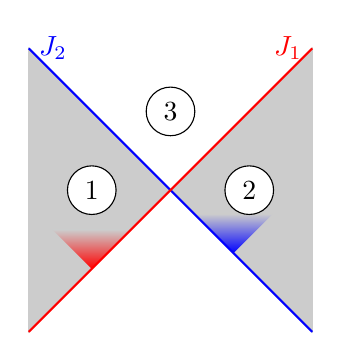
\begin{tikzpicture}
%light cone
\filldraw[black!20] (-1.8,1.8) -- (-1.8,-1.8) -- (1.8,1.8)  -- (1.8,-1.8) -- cycle;

%lightcones
\shade[bottom color=red, top color=black!20] (-1,-1) -- (-0.5,-0.5) -- (-1.5,-0.5) -- cycle;
\shade[bottom color=blue, top color=black!20] (0.8,-0.8) -- (0.3,-0.3) -- (1.3,-0.3) -- cycle;

%\shade[bottom color=red, top color=transparent] (0.3,0.3) -- (0.8,0.8) -- (-0.2,0.8) -- cycle;
%\shade[bottom color=blue] (-0.2,0.2) -- (0.3,0.7) -- (-0.7,0.7) -- cycle;

%axes
%\draw[->,gray!80,thick] (-2,0) -- (2,0) node[below] {$x^1$};
%\draw[->,gray!80,thick] (0,-2) -- (0,2) node[left] {$x^0$}; 
\draw[thick,blue] (1.8,-1.8) -- (-1.8,1.8) node[right] {$J_2$};
\draw[thick,red] (-1.8,-1.8) -- (1.8,1.8) node[left] {$J_1$};



%text
\draw (0,1) node[circle,fill=white,draw=black] {$3$};
\draw (-1,0) node[circle,fill=white,draw=black] {$1$};
\draw (1,0) node[circle,fill=white,draw=black] {$2$};
\end{tikzpicture}